\documentclass[25pt, a0paper, portrait]{tikzposter}
\usepackage[T1]{fontenc}
\renewcommand*\familydefault{\sfdefault}
\usepackage{sfmath}
\usepackage{amsmath}
\usepackage{lipsum}
\usepackage[compress]{cite}
\usepackage{graphicx}

\newcommand{\CORE}{The CORE collaboration}
\newcommand{\PLANCK}{The Planck collaboration}
\newcommand{\prd}{PRD}
\newcommand{\prr}{PRR}
\newcommand{\mnras}{MNRAS}
\newcommand{\jcap}{JCAP}
\newcommand{\jmap}{JMAP}
\newcommand{\joss}{JOSS}
\newcommand{\pasa}{PASA}
\newcommand{\aap}{A\&A}
\newcommand{\prl}{PRL}
\newcommand{\arxiv}{arXiv}
\newcommand{\polychord}{\texttt{PolyChord}}



\makeatletter
\renewcommand\TP@maketitle{%
    \centering
    \vspace{-40pt}
    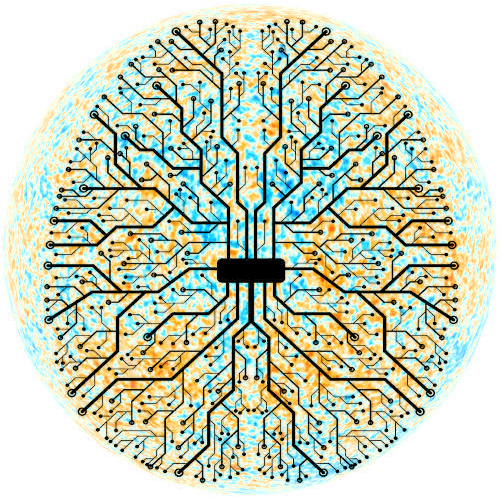
\includegraphics[height=0.11\textwidth]{handley-lab.png}\hfill
    \begin{minipage}[b]{0.7\linewidth}
        \centering
        \color{titlefgcolor}
        {\Huge \sc \@title \par}
        \vspace*{1em}
        {\huge \@author \par}
        \vspace*{1em}
        {\LARGE \@institute}
    \end{minipage}%
    \hfill
\includegraphics[height=0.11\textwidth]{cambridge-cropped.pdf}
}
\makeatother

\title{Clustering Considerations for Nested Sampling}
\author{Adam Ormondroyd <ano23@cam.ac.uk>}
\institute{Kavli Institute for Cosmology $\cdot$ Cavendish Laboratory $\cdot$  University of Cambridge}
%\usetheme{Default}
%\usetheme{Rays}
%\usetheme{Basic}
%\usetheme{Simple}
\usetheme{Envelope}
%\usetheme{Wave}
%\usetheme{Board}
%\usetheme{Autumn}
%\usetheme{Desert}

\tikzposterlatexaffectionproofoff{}

\let\oldbibliography\thebibliography
\renewcommand{\thebibliography}[1]{\oldbibliography{#1}
\setlength{\itemsep}{-5pt}} %Reducing spacing in the bibliography.

\pdfinclusioncopyfonts=1 % Fix fonts on non-linux machines

\usepackage{xcolor}
\definecolor{C0}{HTML}{E06C75}
\definecolor{C1}{HTML}{56B6C2}
\definecolor{C2}{HTML}{56B6C2}
\definecolor{C3}{HTML}{98C07B}
\definecolor{C4}{HTML}{9467bd}
\definecolor{C5}{HTML}{8c564b}
\definecolor{C6}{HTML}{e377c2}
\definecolor{C7}{HTML}{7f7f7f}
\definecolor{C8}{HTML}{bcbd22}
\definecolor{C9}{HTML}{17becf}
\newcommand\C[2][1]{\textcolor{C#1}{#2}}


%\usecolorstyle[colorOne=blue, colorTwo=gray, colorThree=green]{Default}
%\usecolorpalette{BlueGrayOrange}
%\usecolorstyle[colorOne=blue]{mystyle}
%\colorlet{backgroundcolor}{C1}

%% Background Colors
\colorlet{backgroundcolor}{C0!50!white}
\colorlet{framecolor}{black}
%% Title Colors
\colorlet{titlefgcolor}{white}
\colorlet{titlebgcolor}{C0}
%% Block Colors
\colorlet{blocktitlebgcolor}{C0}
\colorlet{blocktitlefgcolor}{white}
\colorlet{blockbodybgcolor}{white}
\colorlet{blockbodyfgcolor}{black}
%% Innerblock Colors
\colorlet{innerblocktitlebgcolor}{C1}
\colorlet{innerblocktitlefgcolor}{black}
\colorlet{innerblockbodybgcolor}{C1!10!white}
%\colorlet{innerblockbodyfgcolor{black}
%% Note colors
\colorlet{notefgcolor}{black}
\colorlet{notebgcolor}{C2!50!white}
\colorlet{notefrcolor}{C2}

\usepackage[hidelinks]{hyperref}
\hypersetup{
    colorlinks,
    linkcolor={C3!50!black},
    citecolor={C3!80!black},
    urlcolor={C3!80!black}
}

\begin{document}
\maketitle

    \block{}{%
        \centering
        
\includegraphics[height=0.09\textwidth]{kicc}
        \hspace{20pt}
        \begin{minipage}[b]{0.73\textwidth}
            Clustering algorithms are integral to multi-modal nested sampling, for both region-based samplers such as \texttt{MultiNest}, and chain-based samplers such as \polychord. Robust identification clusters of live points is crucial for effective spawning of new live points, prior volume estimation and therefore the total evidence calculation. Reliable cluster detection also allows the calculation of the sub-evidences of each cluster, which may correspond to different physical phenomena.
            We have explored extensions to the clustering approach within \polychord, and found that one must not neglect the correlation between the volume estimates of posterior modes corresponding to each cluster during live point generation. We show how different clustering methods affect a reconstruction of the cosmological primordial matter power spectrum $\mathcal P_\mathcal R(k)$.
        \end{minipage}%
        \hspace{20pt}
        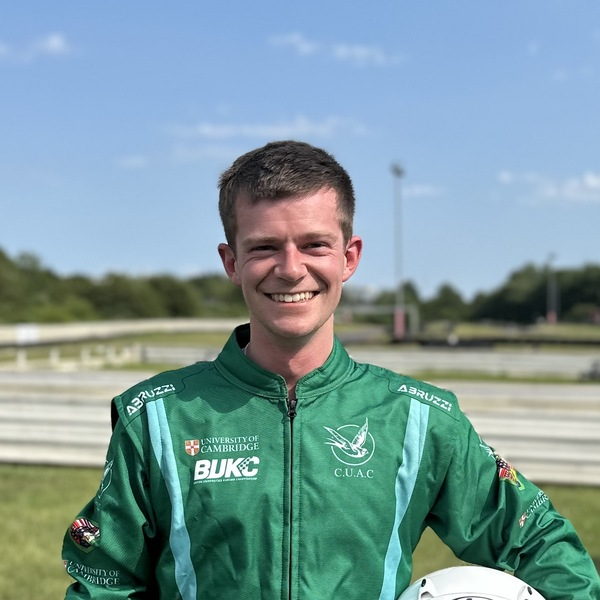
\includegraphics[height=0.09\textwidth]{images/adam_ormondroyd}

    }
\begin{columns}
    \column{0.5}

    \block{The first text box}{%
        \begin{tikzfigure}[The first figure caption]
        \includegraphics[height=0.13\textwidth]{images/image_5}
        \end{tikzfigure}
        \vspace{0.5em}
        \LaTeX is a high-quality typesetting system, it is excellent at mathematics, such as the equation of a circle $x^2 + y^2 = r^2$.
        \begin{center}
            \begin{tabular}{|ll|}
                \hline
                $A$: & The first letter of the roman alphabet. \\
                $\Omega$: & The last letter of the greek alphabet. \\
                \hline
            \end{tabular}
        \end{center}
        \vspace{0.5em}

        Here is Bayes theorem:
        \begin{equation}
            P(A|B) = \frac{P(B|A)P(A)}{P(B)}
            \nonumber
        \end{equation}
    }

    \block{Application to cosmological $\mathcal P_\mathcal R(k)$}{%

        \begin{minipage}{0.22\textwidth}
            \innerblock{\rule[-0.6ex]{0pt}{2.5ex}K-nearest-neighbours}{
                \centering
                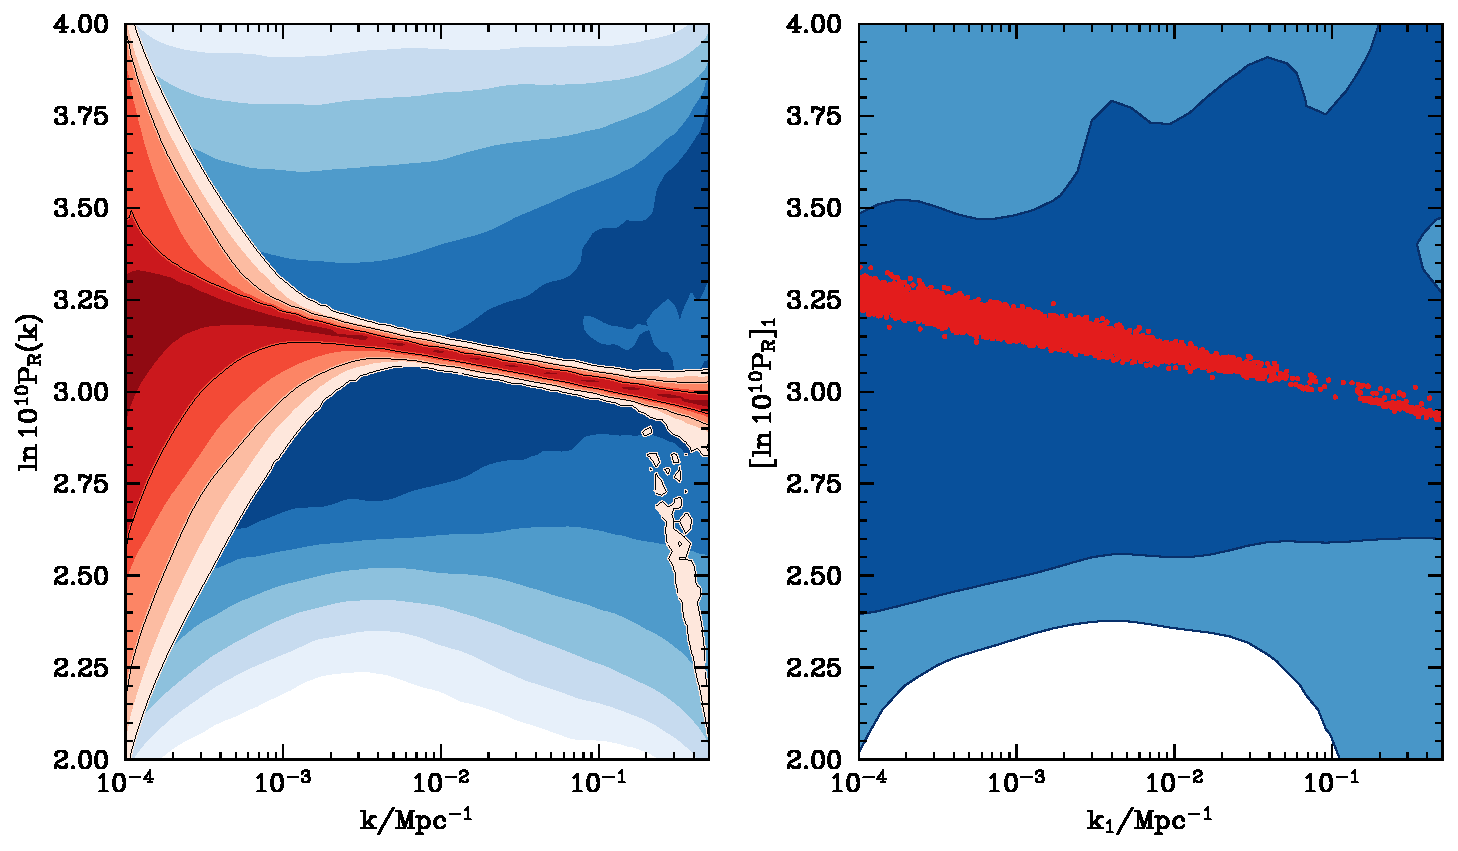
\includegraphics[width=0.9\textwidth]{images/amsterdam/knn}
            }
        \end{minipage}
        \hfill
        \begin{minipage}{0.22\textwidth}
            \innerblock{\rule[-0.6ex]{0pt}{2.5ex}X-means}{
                \centering
                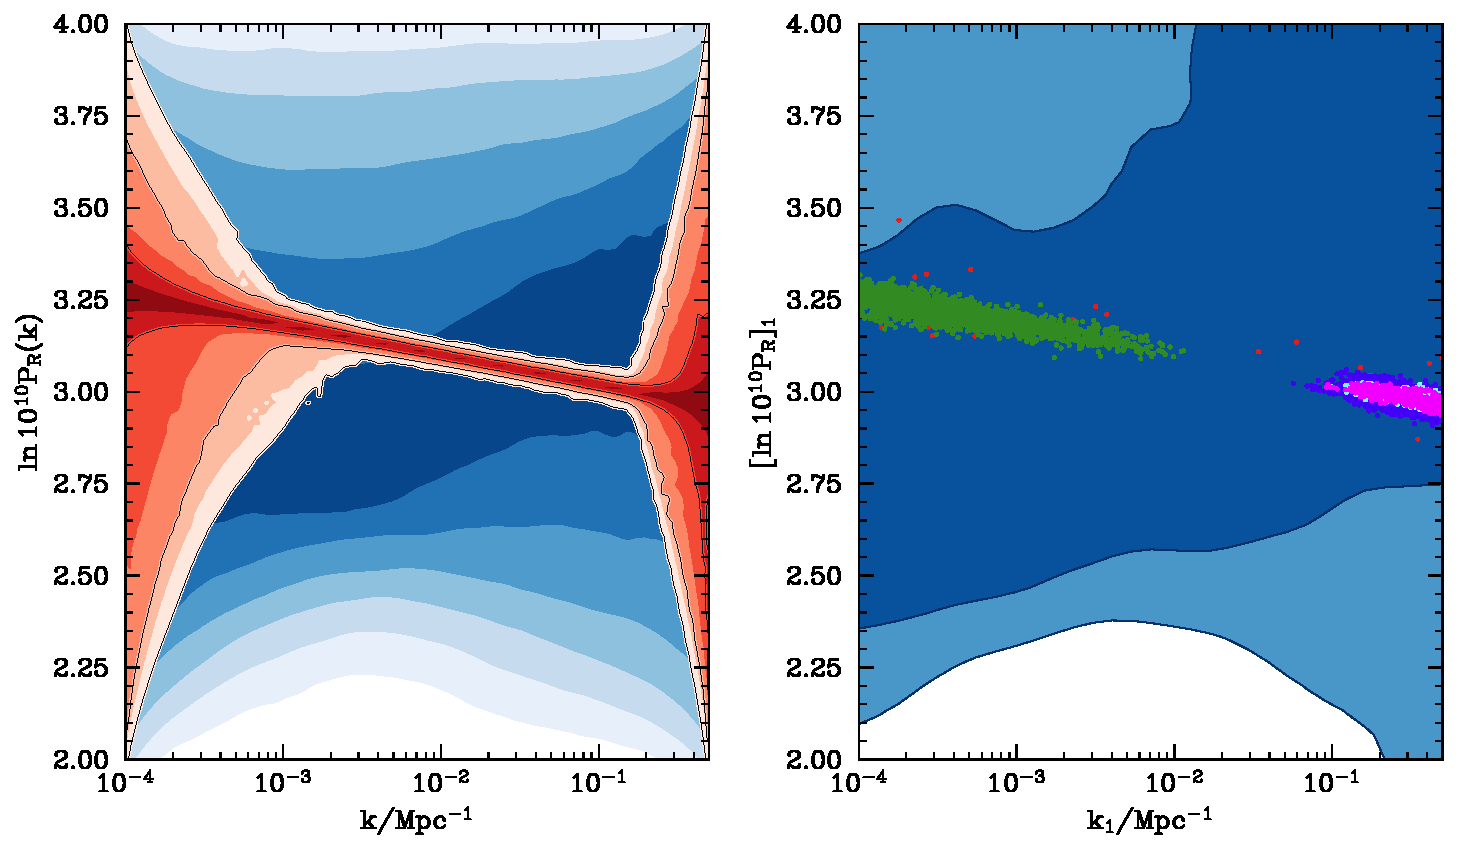
\includegraphics[width=0.9\textwidth]{images/amsterdam/xmeans}
            }
        \end{minipage}
        \begin{minipage}{0.22\textwidth}
            \innerblock{\rule[-0.6ex]{0pt}{2.5ex}DBSCAN}{
                \centering
                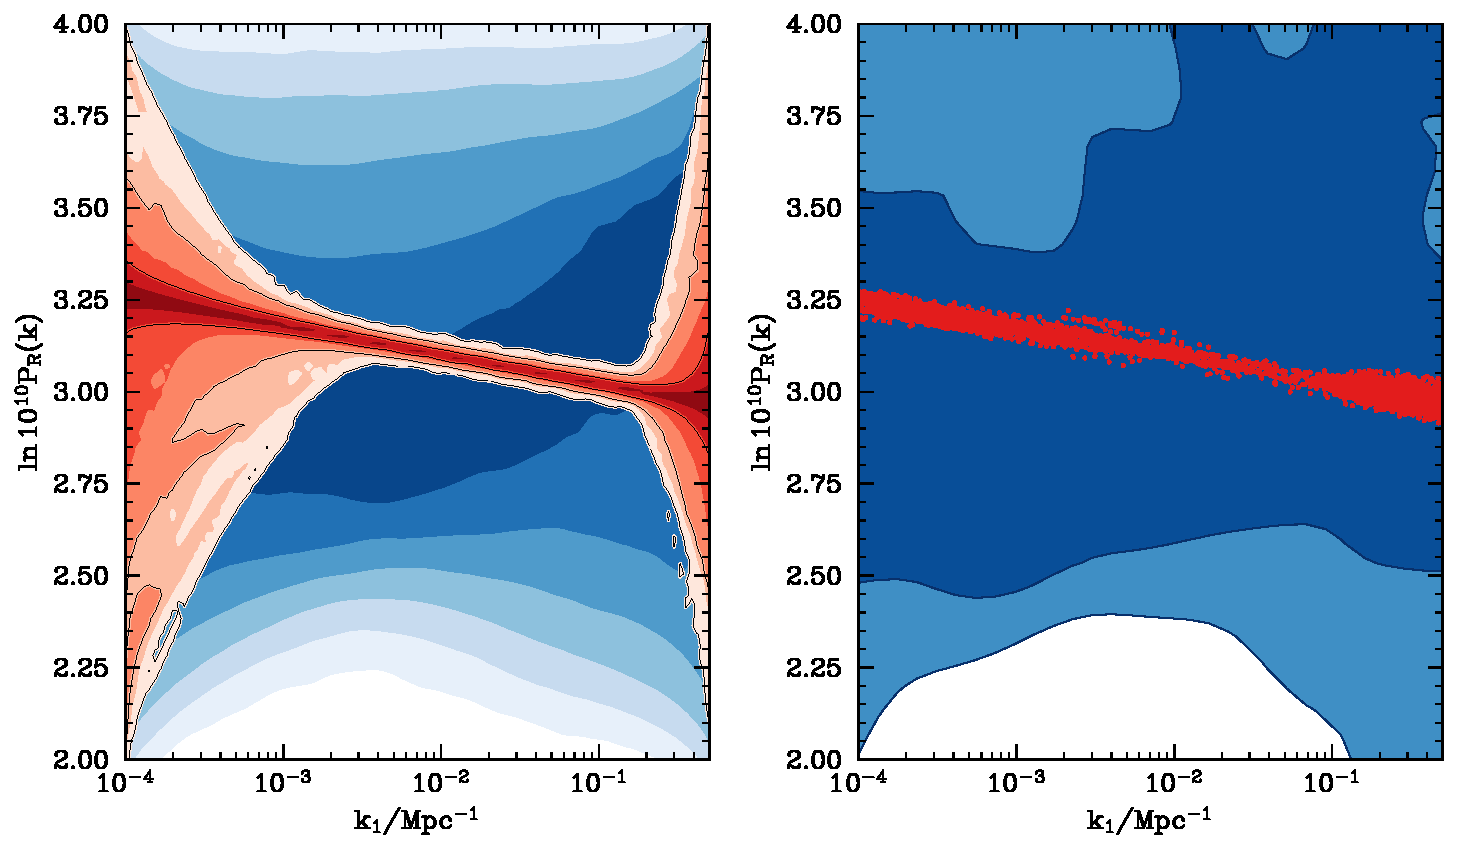
\includegraphics[width=0.9\textwidth]{images/amsterdam/dbscan}
            }
        \end{minipage}
        \hfill
        \begin{minipage}{0.22\textwidth}
            \innerblock{\rule[-0.6ex]{0pt}{2.5ex}using $\mathcal L$ information}{
                \centering
                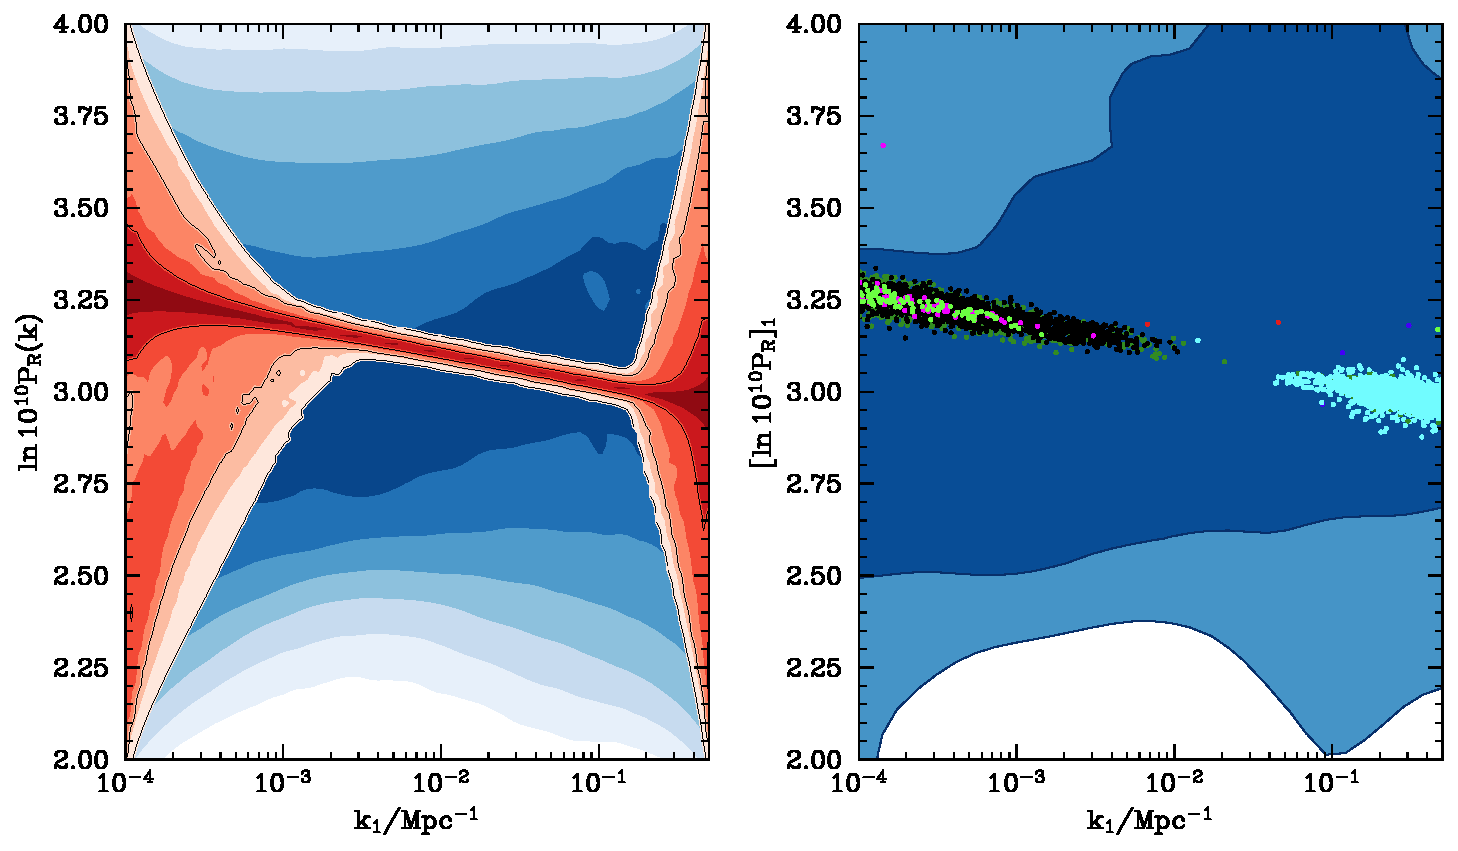
\includegraphics[width=0.9\textwidth]{images/amsterdam/convex}
            }
        \end{minipage}
    }

    \block{BibTeX}{%
        As it is \LaTeX, you can use BibTeX to manage your references. You can also use BibTeX to manage the references in the bibliography.}
    \block{Printing your poster}{
        You can print your poster same day (although don't leave it this late!) at the University Print Shop. I recommend a0, portrait, lightweight cloth (which can be gently folded in a suitcase)
        \href{https://www.pdn.cam.ac.uk/other-pages/avmg/posters}{www.pdn.cam.ac.uk/other-pages/avmg/posters}
    }





    \column{0.5}

    \block{Classes of Nested Sampler}{
        Nested sampling algorithms differ in how they sample new points from the prior, forming two main categories:\\
        \begin{minipage}{0.22\textwidth}
            \innerblock{Chain-based}{
                Taking a sufficiently long random walk within the likelihood contour from an existing live point will generate a new live point. For example, \polychord first uses the covariance matrix of the live points to whiten the space, then perform's Neal's slice sampling along orthogonal directions in that space. \texttt{dynesty} also implements both Neal's and Hamiltonian slice sampling, along with uniform sampling and random walks.

                With multiple modes, contour whitening is ineffective, and a strategy is required to decide from which mode to sample since a random walk restricted by the likelihood contour will never reach another mode. \polychord, after identifying its clusters, picks one of the clusters at random in proportion to its prior volume.
            }
        \end{minipage}\hfill
        \begin{minipage}{0.22\textwidth}
            \innerblock{Region-based}{
                Region-based samplers construct regions around the live points to approximate the likelihood contour, for example \texttt{MultiNest} constructs a series of ellipsoids. These regions are usually expanded by some numerical factor to improve their chances of fully enclosing the likelihood contour, then a point is rejection-sampled from them. The curse of dimensionality means that these techniques are only effective up to $\mathcal O(10)$ dimensions, since the rejection sampling becomes too inefficient, or the expansion factor would have to be so low that significant regions of the likelihood contour would be missed. Multi-modality will also cause inefficiency since the ellipsoids will have to be very large to encompass all modes.
                \\
            }
        \end{minipage}\\
        \vspace{1em}

        \coloredbox{Hybrid method combine the two approaches, in an attempt to alleviate the dimensionality scaling of region-based methods, while reducing the number of likelihood evaluations made outside the contour.}

    }

    \block{Gallery}{%
        \centering
            \includegraphics[height=0.1\textwidth]{images/image_9}%
            \includegraphics[height=0.1\textwidth]{images/image_17}%
            \includegraphics[height=0.1\textwidth]{images/image_12}%
            \includegraphics[height=0.1\textwidth]{images/image_11}\\
            \includegraphics[height=0.1\textwidth]{images/image_14}%
            \includegraphics[height=0.1\textwidth]{images/image_15}%
            \includegraphics[height=0.1\textwidth]{images/image_16}%
            \includegraphics[height=0.1\textwidth]{images/image_18}%
        %\includegraphics[height=0.095\textwidth]{images/image_2}%
        %\includegraphics[height=0.095\textwidth]{images/image_3}%
        %\includegraphics[height=0.095\textwidth]{images/image_4}%
        %\includegraphics[height=0.095\textwidth]{images/image_6}
        %\includegraphics[height=0.095\textwidth]{images/image_10}
        %\includegraphics[height=0.095\textwidth]{images/image_13}
    }

    \block{Concluding box}{%
        \lipsum[4]
    }

    \renewcommand{\section}[2]{}%
    \block{References}{%
        \begin{minipage}[b]{0.35\textwidth}
            \bibliographystyle{unsrt}
            \tiny
            \bibliography{poster}
        \end{minipage}%
        
\includegraphics[width=0.1\textwidth]{QR.png}
    }

    \note[targetoffsetx=0.18\textwidth,targetoffsety=0.04\textwidth, connection,angle=135,radius=0.08\textwidth]{scan here for cool plots and gifs demonstrating clustering!}
\end{columns}
\end{document}
